\documentclass[a4paper,11pt]{article}
\usepackage{fontspec}
\setmainfont{Noto Serif CJK SC}
\XeTeXlinebreaklocale "zh"
\XeTeXlinebreakskip=0pt plus 1pt
\usepackage[margin=24mm]{geometry}
\usepackage{amsmath,booktabs,graphicx}
\title{Anscombe 第 2 组的一阶与二阶拟合：固定留一比较}
\author{Pi Research 本地技术复现记录}
\date{2026 年 9 月}
\begin{document}
\maketitle

\begin{abstract}
本文使用 R 官方 \texttt{datasets::anscombe} 中第 2 组的 11 个观测，记录一个可回查的模型比较。预先固定的评估是 11 折留一：每折在其余 10 点上拟合，并预测被留出的 1 点。一阶模型的留一均方误差为 $2.2041810363$，二阶模型为 $3.1116060757\times10^{-6}$；后者达到事先声明的相对误差阈值。两次正式运行和停止决定均留有独立批准与固定源码。本结果只描述这 11 个已知点上的留一评估，不是独立数据上的预测能力或原论文完整结论的验证。
\end{abstract}

\section{来源与问题}
Anscombe 的论文\cite{anscombe1973}说明单凭汇总统计可能漏掉数据形态差异。本记录只使用 R 官方数据集\cite{rdata}中已经固定的第 2 组数值；未取得并通读原论文全文。数据源文件 SHA-256 为
\begin{center}
{\footnotesize\texttt{02f29379f282fcf909ff988b3fde2be2d5591975ba27ed0efd8714a91629223e}}。
\end{center}
我们检验一个更窄的问题：在同一组 11 点和相同留一规则下，把多项式阶数从 1 改成 2，是否能使均方误差至少下降 10\%。阶数 2 是看过该组数据形态后提出的候选，不能把这次评估当作未参与选模的外部测试。

\section{固定方法}
对 $d\in\{1,2\}$ 和每个观测 $i$，以其余 10 点的最小二乘拟合得到 $\hat f_{d,-i}$；主指标定义为
\begin{equation}
  \operatorname{MSE}_{\mathrm{LOO}}(d)
  =\frac{1}{11}\sum_{i=1}^{11}\bigl(y_i-\hat f_{d,-i}(x_i)\bigr)^2.
\end{equation}
训练集 MSE 仅作辅助描述。两个容器运行使用相同的 R 原始文件、解析程序、比较程序、11 折规则和运行契约，仅配置 \texttt{degree} 不同；各自归档指标与逐点预测。图~\ref{fig:group2} 由另一项单独批准的隔离作业读取这四件固定运行产物绘制，图形产物及其输入摘要在成果包中回查。

\begin{figure}[htbp]
\centering
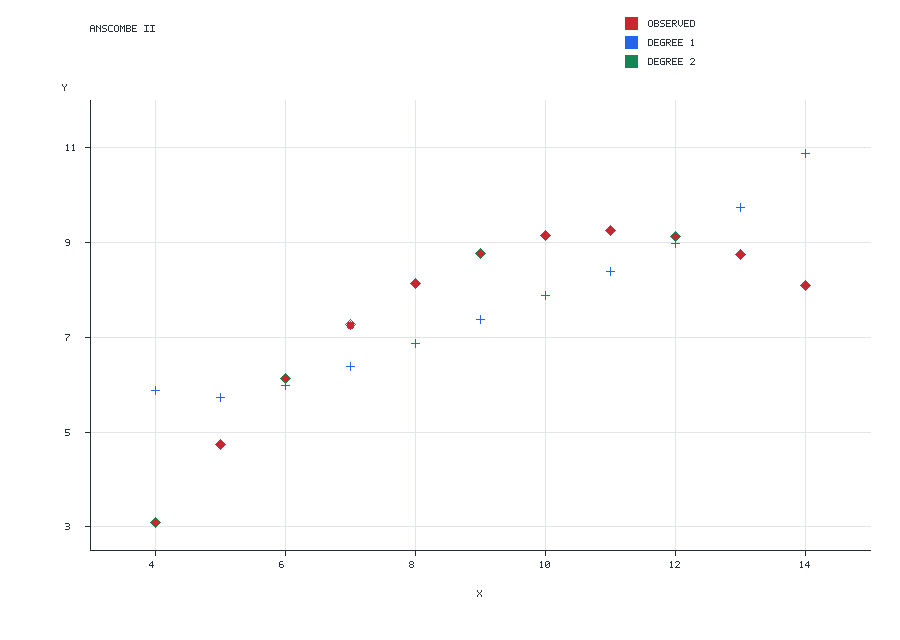
\includegraphics[width=0.91\linewidth]{figure.png}
\caption{第 2 组的 $x$--$y$ 点位。红色是 11 个实际观测，蓝色是一阶模型的逐点留一预测，绿色是二阶模型的逐点留一预测；同一行使用同一个 $x$。此图展示固定产物，不代表外部验证。}
\label{fig:group2}
\end{figure}

\section{结果与停止}
\begin{table}[htbp]
\centering
\caption{两次实际归档的均方误差。两种拟合的观测数均为 11。}
\begin{tabular}{lrr}
\toprule
模型 & 留一均方误差 & 训练集均方误差 \\
\midrule
一阶 & $2.2041810363$ & $1.2523900826$ \\
二阶 & $3.1116060757\times10^{-6}$ & $2.0343293071\times10^{-6}$ \\
\bottomrule
\end{tabular}
\end{table}
二阶与一阶的主指标比为 $1.4116835343\times10^{-6}$，低于预设上限 $0.9$。研究活动因此记录“在这 11 点的留一评估中达到阈值”，再经单独批准停止，不自动追加候选。系统中的科研判断仍需研究者审阅；运行成功、批准和误差变化均不能单独证明更广的科学主张。

\section{可复现范围与局限}
一阶 Run 为 \texttt{01982d5c-5696-45b8-b9ad-f0d0da384ebe}，二阶 Run 为 \texttt{73ccf6f6-7993-43ae-bacf-147113aa66ff}；已停止活动为 \texttt{f63df7ca-807c-4041-8a86-739cc2a37db9}。成果包保留固定源、两份逐点预测、图形生成脚本与输入、可编辑的本 \TeX{} 文件及其编译 PDF。

本比较没有独立外部数据，也没有为模型选择提供与这 11 点无关的测试集。二阶在这里的误差较小不能外推到其他样本、其他组或其他研究问题。本文是由验收夹具撰写的可编辑技术记录，编译、图形核验和报告有效性以产品后续作业的真实记录为准；文稿本身不冒充 Pi 生成或独立科研审查。

\begin{thebibliography}{9}
\bibitem{anscombe1973} F. J. Anscombe, ``Graphs in Statistical Analysis,'' \emph{The American Statistician}, 1973. DOI: 10.1080/00031305.1973.10478966.
\bibitem{rdata} R Core Team, \texttt{datasets::anscombe}, R 官方数据集及源文件；本记录使用的版本按上方 SHA-256 固定。
\end{thebibliography}
\end{document}
